\documentclass{article}
\usepackage{graphicx}
\usepackage{float}
\parskip=12pt

\begin{document}

\title{Laboratory 2: DC and AC Circuits}
\date{October 29, 2014}
\author{Calvin Chan\\304144970\\Physics 4BL Lab 8\\Partners: Caleb Choi, Stanley
Chan}

\maketitle

\section{Introduction}
This lab analyzes the properties of DC and AC circuits by examining the basic
properties of resistors, diodes, capacitors, and inductors and constructing the
two circuits with said components. The lab will examine the current-voltage
characteristics of various load devices – the lab will look at resistors
(individually, in series, and in parallel) and diodes, whereas the AC portion of
the lab, specifically, will also look at two reactive components: capacitors and
inductors.

\section{Experimental Results}

\subsection{DC Circuits: Ohm's Law}

\begin{enumerate}
    \item Build a circuit with two resistors in series, one with a known
    resistance value and another with an unknown value.
    \item Connect a voltage meter to measure the voltage drops through both
    resistors.
    \item Connect the circuit to the ADC. Apply a max voltage of 5V and retrieve
    a sample size of 1,000 points using a sampling rate of 5000 samples/sec.
\end{enumerate}

For the first part of the lab, we want to analyze the current-voltage
characteristic of a single resistor as our load device. We can use an IV curve
to track how much current flows through the resistor at varying voltages, and
thus, verifying Ohm's law \textbf{(eq. \ref{ohms_law})} by generating an IV
curve for the simple resistor \textbf{(fig. \ref{ivcurve_simpleresistor})}. 

\begin{equation}
    \label{ohms_law}
    I(V) = \frac{V}{R}
\end{equation}

\begin{figure}[H]
    \centering
    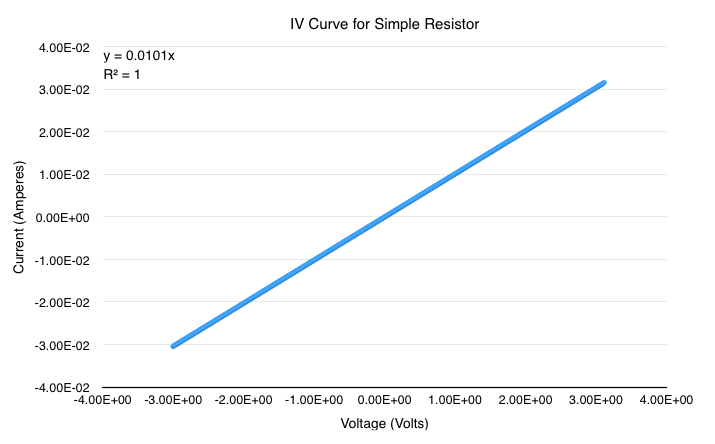
\includegraphics[width=\textwidth]{charts/ivcurve_simpleresistor}
    \caption{IV Curve for a resistor of unknown resistance}
    \label{ivcurve_simpleresistor}
\end{figure}

We used a known resistor of 98.8 $\Omega$ and connected it in series with
another resistor of unknown resistance. Using Ohm's law \textbf{(eq.
\ref{ohms_law})}, the current through the entire circuit was calculated at each
varying voltage.

\subsection{DC Circuits: Deviation from Ohm's Law}

\begin{enumerate}
    \item Build a circuit with a resistor and a diode connected in series.
    \item Connect a voltage meter to measure the voltage drops through both, the
    resistor and the diode.
    \item Connect the circuit to the ADC. Apply a max voltage of 5V and retrieve
    a sample size of 1,000 points using a sampling rate of 5000 samples/sec.
\end{enumerate}

Next, we want to analyze the current-voltage characteristic of a diode as our
load device. We can use an IV curve to track how much current flows through the
diode at varying voltages. Unlike resistors, diodes only allow current to flow
in a single direction when a tiny voltage is applied. 

For this part of the lab, we used a known resistor of 98.8 $\Omega$ and
connected it in series with a diode. Using Ohm's law \textbf{(eq.
\ref{ohms_law})}, the current through the entire circuit was calculated at each
varying voltage.

\begin{figure}[H]
    \centering
    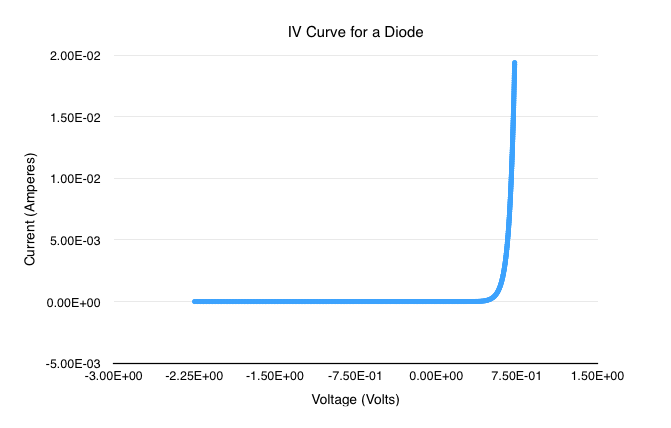
\includegraphics[width=\textwidth]{charts/ivcurve_diode}
    \caption{IV Curve for a diode}
    \label{ivcurve_diode}
\end{figure}

\subsection{AC Circuits: RC Transient State}

\begin{enumerate}
    \item Select a resistor and capacitor and connect them in series.
    \item Ensure that the selecte resistor and capacitor yield a time constant
    of roughly $10^{-3}$ seconds.
    \item Use a voltage generator to generate a voltage with a square waveform
    with a frequency of roughly $10 Hz$ and a voltage amplitude of about $2 V$.
    \item Use the voltmeter to measure the voltage drop across the resistor and
    the capacitor
\end{enumerate}

For this part of the lab, we want to analyze the transient states of a circuit
that involves uses a capacitor load device. We can monitor the input voltage and
compare it to the voltage drop across the capacitor over time, as shown in
\textbf{fig. (\ref{rccurve_transient})}.

\begin{figure}[H]
    \centering
    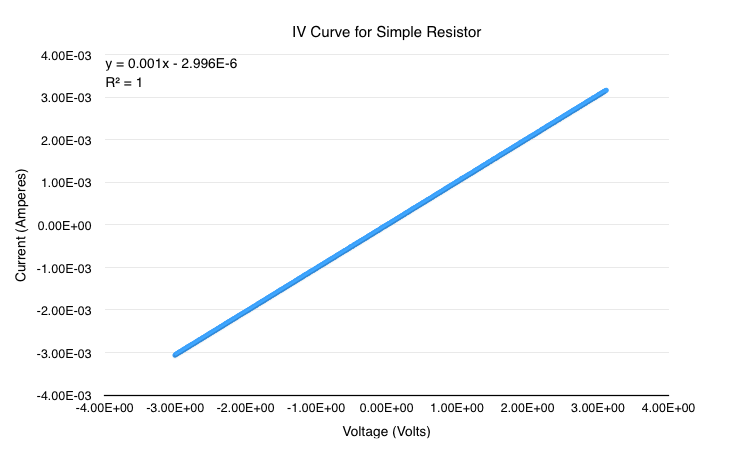
\includegraphics[width=\textwidth]{charts/rccurve_transient}
    \caption{Voltage across the capacitor during the transient state period}
    \label{rccurve_transient}
\end{figure}

We used a known resistor of 1000 $\Omega$ and connected it in series with
a capacitor of 1 $\mu F$.

\subsection{AC Circuits: RL Transient State}

\begin{enumerate}
    \item Build a circuit with a resistor and a diode connected in series.
    \item Connect a voltage meter to measure the voltage drops through both, the
    resistor and the diode.
    \item Connect the circuit to the ADC. Apply a max voltage of 5V and retrieve
    a sample size of 1,000 points using a sampling rate of 5000 samples/sec.
\end{enumerate}

\begin{figure}[H]
    \centering
    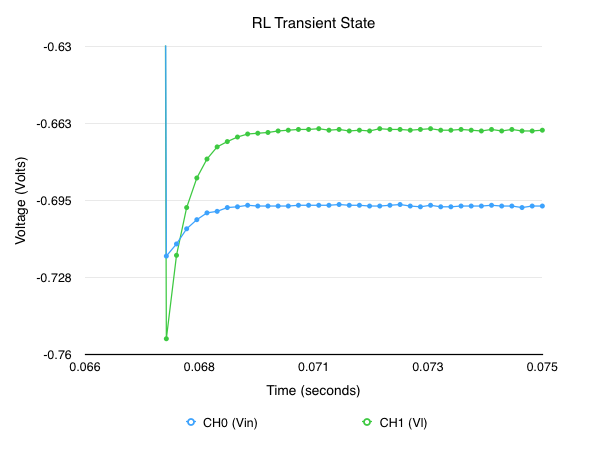
\includegraphics[width=\textwidth]{charts/rlcurve_transient}
    \caption{Voltage across the inductor during the transient state period}
    \label{rlcurve_transient}
\end{figure}

\subsection{AC Circuits: RLC Resonance}

\section{Analysis}

\subsection{DC Circuits: Ohm's Law}

The range of the IV Curve \textbf{(fig. \ref{ivcurve_simpleresistor})} contains
the current values (in Amperes) per domain value, the voltage (in Volts)
measured across the unknown resistor. As such, the curve displays a linear
relationship between the current and voltage, successfully verifying Ohm's law
and proving that voltage and current are directly proportional.

\subsection{DC Circuits: Deviation from Ohm's Law}

The range of the IV Curve for a diode \textbf{(fig. \ref{ivcurve_diode})}
contains the current values (in Amperes) per domain value, the voltage (in
Volts) measured across the diode. From the graph, we can see that diodes deviate
from Ohm's law \textbf{(eq. \ref{ohms_law})} because voltage and current are not
directly proportional through the graph. In fact, the diodes are a non-ohmic
load device that follow a different set of laws altogether; the current that
flows through a diode can be found using the following equation:

\begin{equation}
    \label{iv_diode}
    I(V) = I_{0}(e^{e^{\frac{|e|V}{nk_{B}T}}}-1)
\end{equation}

\section{Conclusion}
Write your conclusion here.

\end{document}
